
\section{Native Code}
\begin{frame}{Native Code}
    \begin{itemize}
    \item Executable machine code
    \item Communication done via Java Native Interface (JNI) \cite{JNISpecChapter1}
    \item On Android: Native Development Kit (NDK) \cite{AndroidNdkIntro}
    \item Useful for:
    \begin{itemize}
    	\item Performance critical code
    	\item Using platform specific features
    	\item (Re)using native libraries
    \end{itemize}
    \end{itemize}
\end{frame}

\section{Java Native Interface(JNI)}
\begin{frame}{Java Native Interface}
    \begin{itemize}
    \item Enables Java code to interoperate with applications and libraries written in other programming languages 
    \item No security checks performed
    \item Java and Native code are running in the same address space
    \item Native Code is able to read and write arbitrary memory from the JVM
    \end{itemize}
    $\Rightarrow$ Dangerous seen from a security perspective.
\end{frame}

\begin{frame}{Java Native Interface}{Part 2}
    \begin{itemize}
    \item Flaws in native libraries can enable attackers to read and write the JVM's memory \cite[p. 3]{Sun_jvm-portablesandboxing}
    \item JNI allows to retrieve and set the content of private fields. This enables an attacker to steal confidential information \cite[p. 3]{Sun_jvm-portablesandboxing}
    \item JNI allows to set the destination of an object pointer without type-checking. Thus type-confusion attacks are possible \cite[p. 4]{Sun_jvm-portablesandboxing}
    \item Bugs in the Linux kernel can enable an attacker to escalate privileges, like done in 'Dirty Cow' (CVE--2016--5195) \cite{DirtyCow}. Over JNI such attacks can directly be initiated
    \item Changing the behavior of the Java application by replacing functions by manipulating or injecting byte code using code patching methods.
    \end{itemize}
\end{frame}



\begin{frame}[fragile]{Java Native Interface}{Part 3}

Loading native library (in Java):
\begin{lstlisting}[language=Java, style=JavaCodeStyle]
 System.loadLibrary("libName");
\end{lstlisting}

Declaring a native method (in Java):
\begin{lstlisting}[language=Java, style=JavaCodeStyle]
package com.example;
public class Native {
  public native String fromNative();
}
\end{lstlisting}

Defining a native method (in C++):
\begin{lstlisting}[language=C++, style=CppCodeStyle]
extern "C" JNIEXPORT jstring JNICALL
Java_com_example_fromNative(JNIEnv *env,jobject /* this */) {
    const char* msg = "Hello from C++";
    return env->NewStringUTF(msg);
}
\end{lstlisting}

\begin{itemize}
    \item JNIEnv defines the JNI interface methods.
    \item The JNIEnv variable is created by the JVM and a pointer to it is pushed on the callstack as the first parameter
    \end{itemize}

\end{frame}



\section{Android Runtime (ART) Internals}
\begin{frame}{Android Runtime (ART)}
    \begin{itemize}
    \item The managed runtime used by applications and some system services on Android
    $\Rightarrow$ The "JVM" of Android
    \item Replaced Dalvik in Android 5.0 (Lollipop) \footnote{\url{https://developer.android.com/about/versions/android-5.0-changes.html}}
    \item Introduced Ahead-of-time (AOT) compilation
    \item Android 7.0 (Nougat) reintroduced a JIT Compiler working along with the AOT compiler
    \begin{itemize}
    	\item Only 'hot' methods are compiled Ahead-of-time 
    	\item If a method gets 'hot', it will be compiled by the AOT compiler
    	\item Native methods are not interpreted, 'hotness' count is ignored \newline
    	$\Rightarrow$ In order to replace an existing java method, the method has to be set to native and its 'hotness' count has to be set to 0 (not 'hot')
    \end{itemize}
    \end{itemize}
\end{frame}



\begin{frame}[fragile]{ART JIT}{Part 2}

\begin{figure}[H]
	\begin{center}
	\vspace*{-2cm}
		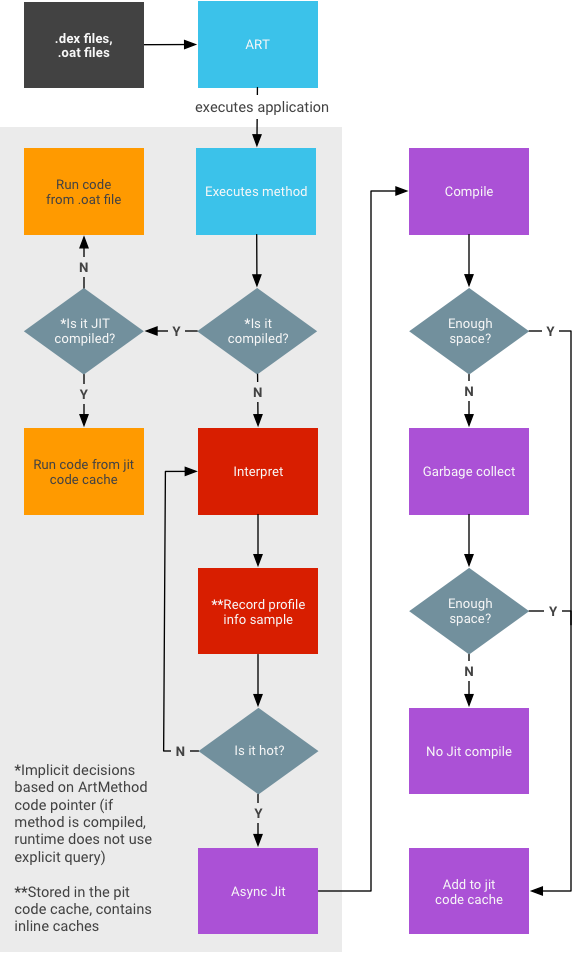
\includegraphics[scale=0.3]{figures/jit-workflow.png}
	\end{center}
	\caption{JIT Workflow on Android 7.0 and above \cite{JitWorkFlow}}
	\label{JitWorkflow}
\end{figure}


\end{frame}


\section{Function Hooking}
\begin{frame}{Function Hooking}
    \begin{itemize}
    \item Intercepts a function and redirects execution flow to another memory address
    \item Established by using a jump or return instructions
    \item Save the original function before modifying it
    \begin{itemize}
    	\item Original function can still be called
    	\item Called trampoline hook
    	\item Technique coined by Micrsoft's Detour library \cite{detours-binary-interception-of-win32-functions}
    \end{itemize}
    \end{itemize}
\end{frame}

%\begin{frame}{Function Hooking (Art)}
%    \begin{itemize}
%    \item The target ArtMethod is set to native (by setting the native flag) \newline
%    $\Rightarrow$ JIT compiler and code profiler don't interfere 
%    
%    \item Established by using a jump or return instructions
 %   \item Save the original function before modifying it
 %   \begin{itemize}
  %  	\item Original function can still be called
   % 	\item Called trampoline hook
    %	\item Technique coined by Micrsoft's Detour library \cite{detours-binary-interception-of-win32-functions}
%    \end{itemize}
%    \end{itemize}
%\end{frame}*/

\begin{frame}[fragile]{Function Hooking (Art)}
    \begin{lstlisting}[language=C++, style=CppCodeStyle, caption=Redirection to another address]
unsigned char redirect[] = {
        0x68, 0x74, 0x56, 0x34 , 0x12, // push   0x12345678 (addr that contains target address)
        0xc3						  //ret	   
};

void source() {}
void target() {}
void foo() {

	void* address = target;	
	
	// set the target address inside redirect
	memcpy(redirect + 1, &address, 4);
	
	//Direct source to target
	memcpy(source, redirect, sizeof(redirect)); 
};
	\end{lstlisting}
\end{frame}

\begin{frame}[fragile]{Back to JNI}

	\begin{itemize}
    	\item Java Methods and classes are mapped to C++ types
    	\item Over JNIEnv, methods and classes can be found by their name (FindClass, GetMethodID)
    	\item The definition of the structures are dependent from the concrete JVM implementation
    \end{itemize}

\begin{lstlisting}[language=C++, style=CppCodeStyle, caption=jmethodID definition in jni.h]
struct _jmethodID;  /* opaque structure */
typedef struct _jmethodID* jmethodID;  /* method IDs */
\end{lstlisting}

	\begin{itemize}
    	\item In Android 8.0.0 (rev. 36) the definition is in art/runtime/art\_method.h \cite{ArtMethodOreoRev36}\newline
    	$\Rightarrow$ jmethodID is actually a pointer to an ArtMethod object!
    \end{itemize}


\end{frame}

\begin{frame}[fragile]{Function Hooking (Art)}{Part 4}

\begin{lstlisting}[language=C++, style=CppCodeStyle, caption=ArtMethod and x86 offsets \cite{ArtMethodOreoRev36},
escapechar=!]
    
class ArtMethod FINAL { 
 protected:
  GcRoot<mirror::Class> declaring_class_; //offset 0
 !\colorbox{yellow}{std::atomic<std::uint32\_t> access\_flags\_;}! //offset 4
  uint32_t dex_code_item_offset_; //offset 8
  uint32_t dex_method_index_; //offset 12
  uint16_t method_index_; //offset 16
  !\colorbox{yellow}{uint16\_t hotness\_count\_;}! //offset 18
  struct PtrSizedFields {
    ArtMethod** dex_cache_resolved_methods_; //offset 20
    !\colorbox{yellow}{void* data\_;}! //offset 24
    !\colorbox{yellow}{void* entry\_point\_from\_quick\_compiled\_code\_;}! //offset 28
  } ptr_sized_fields_;
};
\end{lstlisting}

\end{frame}

\begin{frame}{Function Hooking (Art)}{Part 5}
    \begin{itemize}
    \item  entry\_point\_from\_quick\_compiled\_code\_ is used as the entry point for all methods
    \item data\_ is used for secveral purposes, but for native functions it points to the native code.
    \item access\_flags\_ contains a specific flag for native methods
    \item hotness\_count\_ is not used for native methods 
    \item hotness\_count\_ has to be set to 0 for hooked methods not being native before the method is called
    \end{itemize}
\end{frame}


\begin{frame}[fragile]{Function Hooking (Art)}{Part 6}

\begin{figure}[H]
	\begin{center}
	\hspace*{-1cm}
		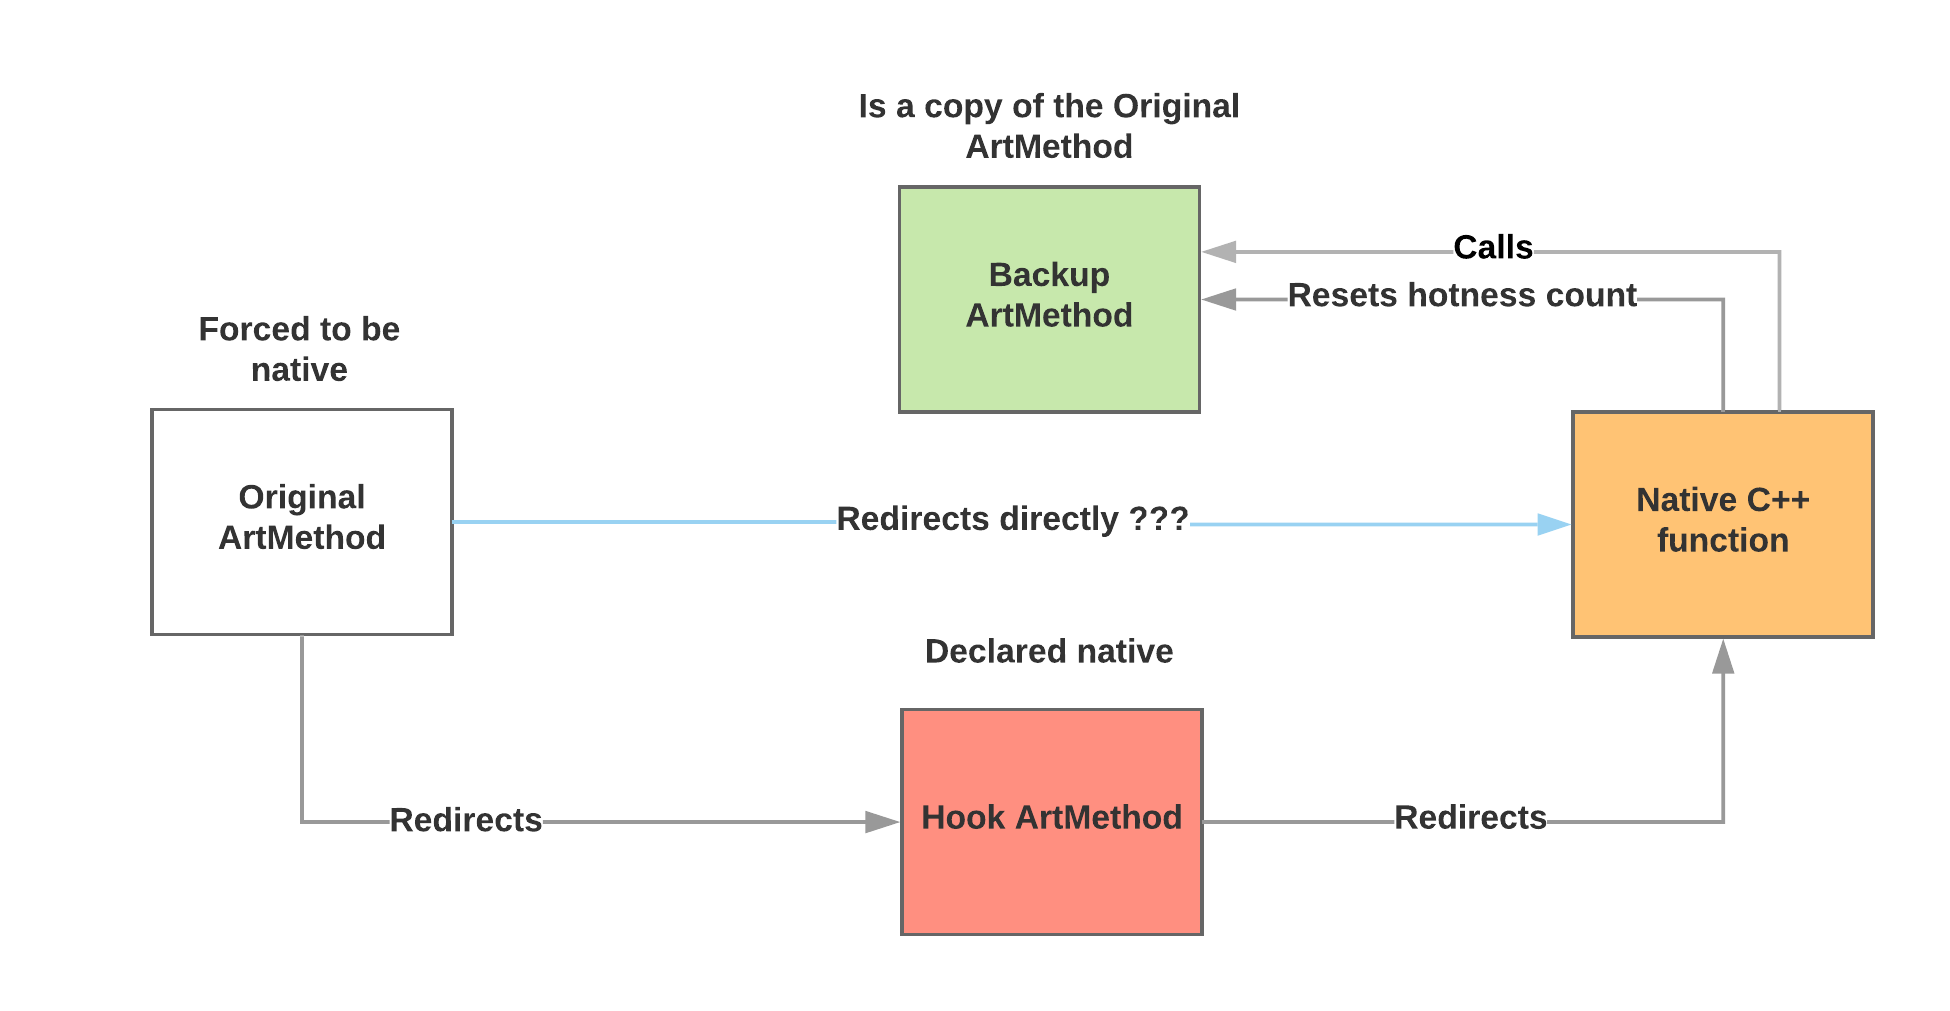
\includegraphics[scale=0.75]{figures/HookProcess.png}
	\end{center}
	\caption{Hooking an Art method}
	\label{HookEndResult}
\end{figure}


\end{frame}

\section{Attack Scenario}
\begin{frame}{Attack Scenario}
Benign App:
    \begin{itemize}
    \item Loads a native library
    \item A simple text messenger 
    \item User can write text messages to a remote server
    \item Communication is encrypted using asymmetric cryptography (TLSv1.2) 
    \end{itemize}
Evil Library:
    \begin{itemize}
    \item Wants to know what is send and received
    \item Downloads helping dex file from evil remote server that contains method declarations for the function hooks
    \item Hooks send and receive methods of the benign app
    \item Changes the content of send and received messages 
    \end{itemize}    
\end{frame}

